\documentclass[11pt]{article}
\usepackage[margin=1in]{geometry}
\usepackage{tikz}
\usetikzlibrary{positioning, shapes.geometric, arrows.meta, fit, backgrounds}
\usepackage{listings}
\usepackage{xcolor}
\usepackage{hyperref}

\title{Cozl-Maidl Family Genealogy Website\\Architecture Documentation}
\author{Next.js 14 Application}
\date{\today}

\begin{document}

\maketitle
\tableofcontents
\newpage

\section{System Overview}

The Cozl-Maidl Family Genealogy Website is a Next.js 14 application that displays family tree information parsed from a GEDCOM file. The application uses server-side rendering for initial page loads and client-side interactivity for search and filtering.

\subsection{Technology Stack}
\begin{itemize}
    \item \textbf{Framework:} Next.js 14.2.0 (React-based)
    \item \textbf{Language:} TypeScript
    \item \textbf{Styling:} Tailwind CSS
    \item \textbf{Data Format:} GEDCOM (Genealogical Data Communication)
    \item \textbf{Parser:} parse-gedcom v2.0.1
    \item \textbf{Deployment Target:} Vercel (static hosting)
\end{itemize}

\section{Architecture Diagram}

\begin{figure}[h]
\centering
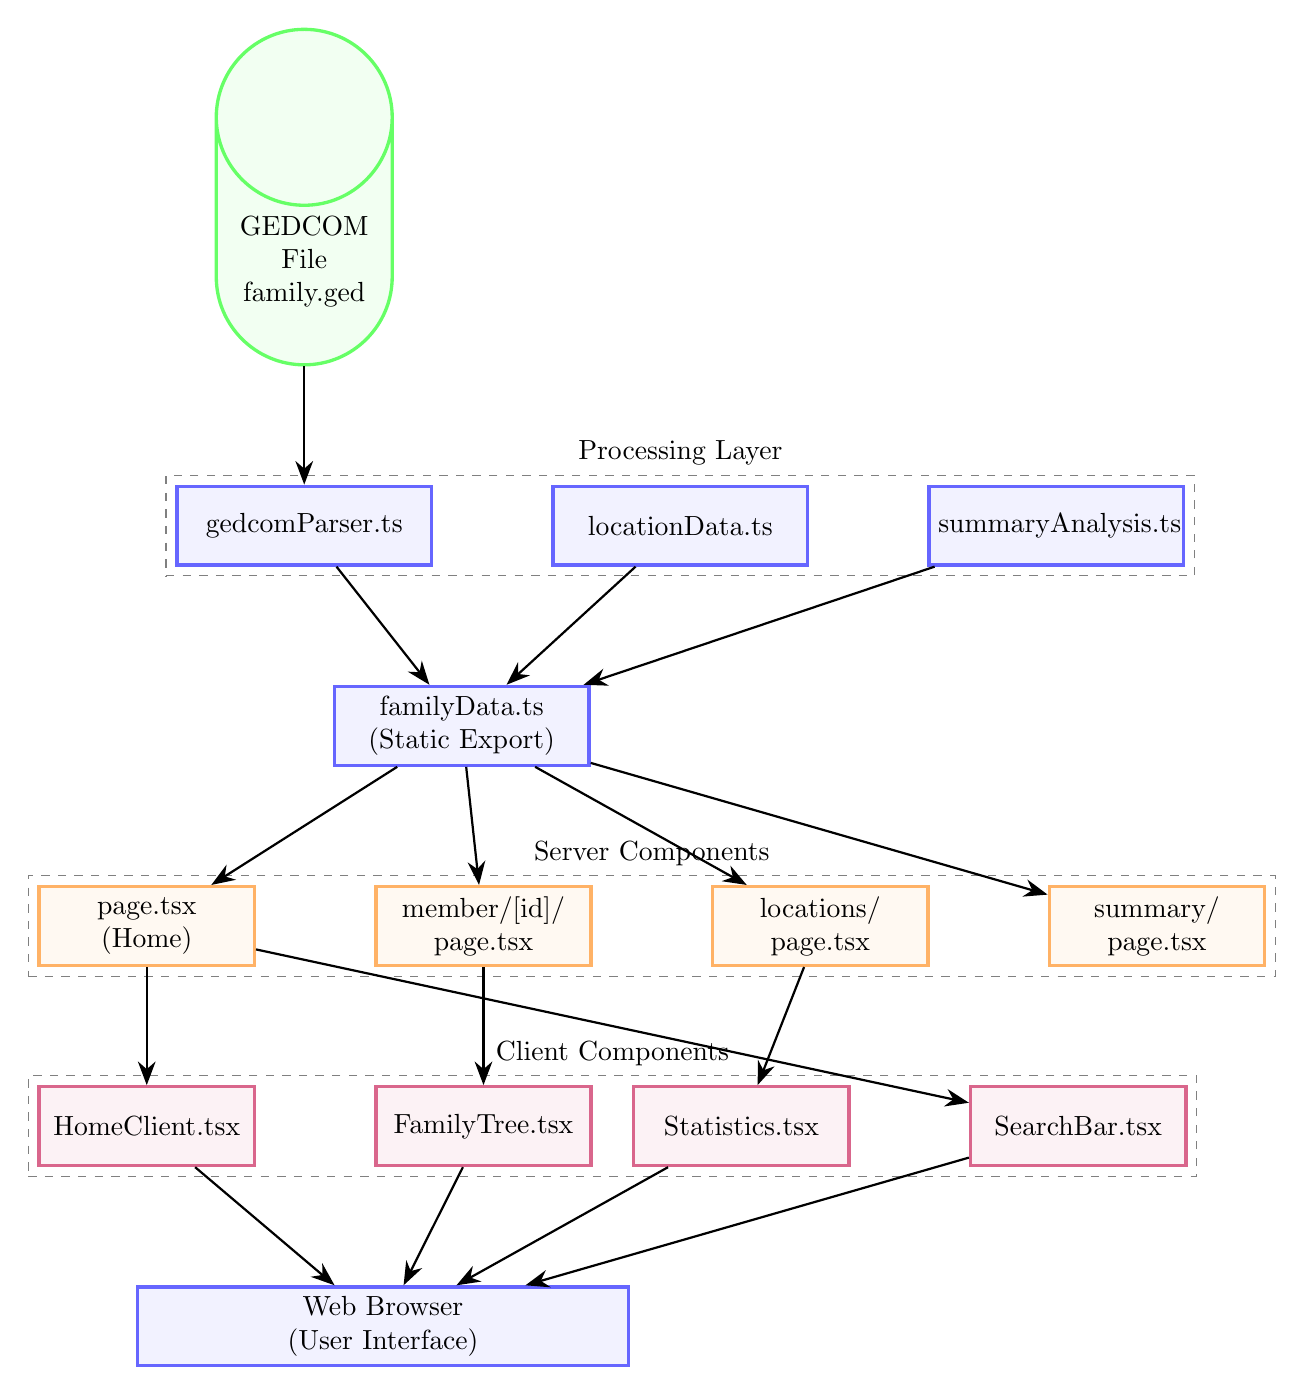
\begin{tikzpicture}[
    node distance=1.5cm,
    component/.style={rectangle, draw=blue!60, fill=blue!5, very thick, minimum height=1cm, text width=3cm, align=center},
    data/.style={cylinder, shape border rotate=90, draw=green!60, fill=green!5, very thick, minimum height=1cm, text width=2cm, align=center},
    page/.style={rectangle, draw=orange!60, fill=orange!5, very thick, minimum height=1cm, text width=2.5cm, align=center},
    client/.style={rectangle, draw=purple!60, fill=purple!5, very thick, minimum height=1cm, text width=2.5cm, align=center},
    arrow/.style={-{Stealth[length=3mm]}, thick}
]

% Data Layer
\node[data] (gedcom) {GEDCOM File\\family.ged};

% Parser Layer
\node[component, below=of gedcom] (parser) {gedcomParser.ts};
\node[component, right=of parser] (location) {locationData.ts};
\node[component, right=of location] (summary) {summaryAnalysis.ts};

% Data Store
\node[component, below=of parser, xshift=2cm] (familydata) {familyData.ts\\(Static Export)};

% Server Pages
\node[page, below=of familydata, xshift=-4cm] (home) {page.tsx\\(Home)};
\node[page, right=of home] (member) {member/[id]/\\page.tsx};
\node[page, right=of member] (locations) {locations/\\page.tsx};
\node[page, right=of locations] (summarypage) {summary/\\page.tsx};

% Client Components
\node[client, below=of home] (homeclient) {HomeClient.tsx};
\node[client, below=of member] (familytree) {FamilyTree.tsx};
\node[client, below=of locations, xshift=-1cm] (stats) {Statistics.tsx};
\node[client, right=of stats] (search) {SearchBar.tsx};

% Browser
\node[component, below=of homeclient, xshift=3cm, text width=6cm] (browser) {Web Browser\\(User Interface)};

% Arrows
\draw[arrow] (gedcom) -- (parser);
\draw[arrow] (parser) -- (familydata);
\draw[arrow] (location) -- (familydata);
\draw[arrow] (summary) -- (familydata);

\draw[arrow] (familydata) -- (home);
\draw[arrow] (familydata) -- (member);
\draw[arrow] (familydata) -- (locations);
\draw[arrow] (familydata) -- (summarypage);

\draw[arrow] (home) -- (homeclient);
\draw[arrow] (member) -- (familytree);
\draw[arrow] (locations) -- (stats);
\draw[arrow] (home) -- (search);

\draw[arrow] (homeclient) -- (browser);
\draw[arrow] (familytree) -- (browser);
\draw[arrow] (stats) -- (browser);
\draw[arrow] (search) -- (browser);

% Background boxes
\begin{scope}[on background layer]
    \node[draw=gray, dashed, fit=(parser) (location) (summary), label=above:Processing Layer] {};
    \node[draw=gray, dashed, fit=(home) (member) (locations) (summarypage), label=above:Server Components] {};
    \node[draw=gray, dashed, fit=(homeclient) (familytree) (stats) (search), label=above:Client Components] {};
\end{scope}

\end{tikzpicture}
\caption{System Architecture - Component Flow}
\end{figure}

\newpage

\section{Component Details}

\subsection{Data Layer}

\subsubsection{GEDCOM File (family.ged)}
The source of truth for all genealogical data. Contains:
\begin{itemize}
    \item 402 individual records (INDI nodes)
    \item 115 family records (FAM nodes)
    \item Birth, death, marriage events
    \item Location information
    \item Relationships (parent-child, spouse)
\end{itemize}

\subsection{Processing Layer}

\subsubsection{gedcomParser.ts}
\textbf{Purpose:} Parse GEDCOM format into TypeScript objects.

\textbf{Key Functions:}
\begin{itemize}
    \item \texttt{parseGedcomFile()}: Main entry point, reads file and parses
    \item \texttt{parseIndividual()}: Extracts person data from INDI nodes
    \item \texttt{parseFamily()}: Extracts family relationships from FAM nodes
\end{itemize}

\textbf{Data Structure:}
\begin{lstlisting}[language=JavaScript, basicstyle=\small\ttfamily]
interface FamilyMember {
  id: string;
  name: string;
  sex?: string;
  birthDate?: string;
  birthYear?: number;
  birthPlace?: string;
  deathDate?: string;
  deathYear?: number;
  deathPlace?: string;
  parentIds: string[];
  spouseIds: string[];
  childrenIds: string[];
  events: Event[];
}
\end{lstlisting}

\subsubsection{locationData.ts}
\textbf{Purpose:} Normalize and deduplicate location names.

\textbf{Key Functions:}
\begin{itemize}
    \item \texttt{getCanonicalLocation()}: Maps variations to standard names
    \item \texttt{getLocationInfo()}: Provides historical context and metadata
\end{itemize}

\textbf{Example Mapping:}
\begin{itemize}
    \item "Madison, Madison, Illinois" → "Madison, Illinois"
    \item "Kolovec, West Bohemia, Czech Republic" (canonical form)
\end{itemize}

\subsubsection{summaryAnalysis.ts}
\textbf{Purpose:} Generate statistical summaries and narrative text.

\textbf{Analyzes:}
\begin{itemize}
    \item Demographics (gender, lifespan averages)
    \item Migration patterns (Czech Republic → USA)
    \item Family sizes and structures
    \item Birth/death decade distributions
    \item Surname frequencies
\end{itemize}

\textbf{Output:} FamilySummary object with narrative paragraphs

\subsection{Data Store Layer}

\subsubsection{familyData.ts}
\textbf{Purpose:} Static export of parsed data for all pages.

\textbf{Exports:}
\begin{lstlisting}[language=JavaScript, basicstyle=\small\ttfamily]
export const familyMembers: FamilyMember[];
export function getMemberById(id: string);
export function getParents(member);
export function getChildren(member);
export function getSpouses(member);
export function getSiblings(member);
\end{lstlisting}

\textbf{Note:} Data is parsed once at build time, then statically served.

\subsection{Server Components Layer}

\subsubsection{page.tsx (Home)}
\textbf{Type:} Server Component

\textbf{Responsibilities:}
\begin{itemize}
    \item Load familyMembers data
    \item Generate FamilySummary
    \item Pass data to HomeClient
\end{itemize}

\textbf{Why Server Component:} No state, just data loading.

\subsubsection{member/[id]/page.tsx}
\textbf{Type:} Server Component with Dynamic Routing

\textbf{URL Pattern:} \texttt{/member/I270043615371}

\textbf{Responsibilities:}
\begin{itemize}
    \item Extract member ID from URL params
    \item Fetch member data and relationships
    \item Render FamilyTree component
    \item Display birth/death information
\end{itemize}

\subsubsection{locations/page.tsx}
\textbf{Type:} Server Component

\textbf{Responsibilities:}
\begin{itemize}
    \item Aggregate locations from all members
    \item Group by canonical location names
    \item Count birth/death occurrences per location
    \item Display with historical context
\end{itemize}

\subsubsection{summary/page.tsx}
\textbf{Type:} Server Component

\textbf{Responsibilities:}
\begin{itemize}
    \item Generate comprehensive family summary
    \item Display narrative paragraphs
    \item Show migration visualization
    \item Present statistical breakdowns
\end{itemize}

\subsection{Client Components Layer}

\subsubsection{HomeClient.tsx}
\textbf{Type:} Client Component ('use client')

\textbf{State:}
\begin{itemize}
    \item searchQuery: string
    \item sortBy: 'name' | 'birthYear'
\end{itemize}

\textbf{Features:}
\begin{itemize}
    \item Hero section with narrative
    \item Search filtering (name, year, place)
    \item Sort controls (name/year)
    \item Member cards grid (402 members)
    \item Statistics integration
\end{itemize}

\textbf{Why Client Component:} Needs useState for search/sort.

\subsubsection{FamilyTree.tsx}
\textbf{Type:} Client Component

\textbf{Purpose:} Visual family tree diagram

\textbf{Display Sections:}
\begin{itemize}
    \item Parents (blue boxes)
    \item Spouses (purple boxes)
    \item Current person (yellow box)
    \item Children (green boxes)
    \item Siblings (gray boxes)
\end{itemize}

\subsubsection{Statistics.tsx}
\textbf{Type:} Client Component

\textbf{Displays:}
\begin{itemize}
    \item Total Family Members
    \item Male/Female ratio
    \item Average Lifespan
    \item Earliest Birth Year
    \item Latest Birth Year
    \item Unique Locations (clickable link)
\end{itemize}

\subsubsection{SearchBar.tsx}
\textbf{Type:} Client Component

\textbf{Props:}
\begin{lstlisting}[language=JavaScript, basicstyle=\small\ttfamily]
interface SearchBarProps {
  onSearch: (query: string) => void;
}
\end{lstlisting}

\textbf{Features:}
\begin{itemize}
    \item Real-time search input
    \item Search icon indicator
    \item Placeholder text guidance
\end{itemize}

\section{Data Flow}

\subsection{Build Time (Static Generation)}

\begin{enumerate}
    \item \textbf{Parse GEDCOM:} gedcomParser.ts reads family.ged
    \item \textbf{Process Data:} Extract individuals and families
    \item \textbf{Normalize:} locationData.ts canonicalizes place names
    \item \textbf{Export:} familyData.ts provides static data
    \item \textbf{Generate Pages:} Next.js pre-renders all routes
    \item \textbf{Output:} Static HTML/CSS/JS files for Vercel
\end{enumerate}

\subsection{Runtime (User Request)}

\begin{enumerate}
    \item \textbf{User visits URL:} Browser requests page
    \item \textbf{Server response:} Next.js serves pre-rendered HTML
    \item \textbf{Hydration:} React attaches client-side interactivity
    \item \textbf{User interaction:} Search/filter updates client-side
    \item \textbf{Navigation:} Next.js Link components for fast routing
\end{enumerate}

\section{Key Design Decisions}

\subsection{Server vs Client Components}

\textbf{Server Components:}
\begin{itemize}
    \item All page.tsx files (no state needed)
    \item Data loading and processing
    \item Better performance (smaller JS bundle)
\end{itemize}

\textbf{Client Components:}
\begin{itemize}
    \item Components with useState/useEffect
    \item Interactive features (search, sort)
    \item Event handlers
\end{itemize}

\subsection{Static Site Generation}

\textbf{Benefits:}
\begin{itemize}
    \item Zero server costs (Vercel free tier)
    \item Instant page loads
    \item Better SEO (pre-rendered HTML)
    \item Simple deployment
\end{itemize}

\textbf{Trade-off:}
\begin{itemize}
    \item Must rebuild to update data
    \item Not suitable for live-updating content
\end{itemize}

\subsection{GEDCOM as Source of Truth}

\textbf{Advantages:}
\begin{itemize}
    \item Standard genealogy format
    \item Compatible with other software
    \item Easy to maintain/update
    \item No database needed
\end{itemize}

\section{Deployment Architecture}

\begin{figure}[h]
\centering
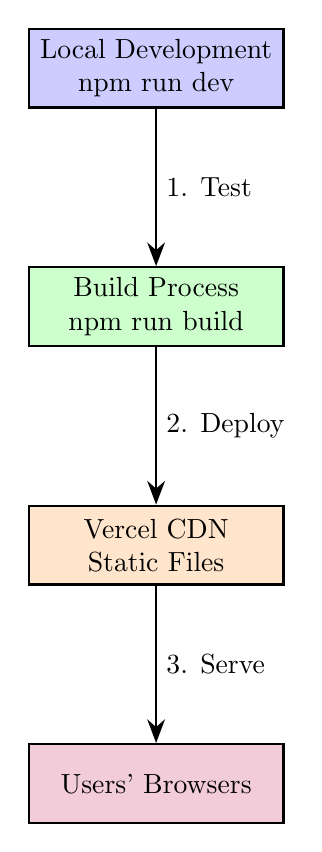
\begin{tikzpicture}[
    node distance=2cm,
    box/.style={rectangle, draw, thick, minimum height=1cm, text width=3cm, align=center}
]

\node[box, fill=blue!20] (local) {Local Development\\npm run dev};
\node[box, fill=green!20, below=of local] (build) {Build Process\\npm run build};
\node[box, fill=orange!20, below=of build] (vercel) {Vercel CDN\\Static Files};
\node[box, fill=purple!20, below=of vercel] (users) {Users' Browsers};

\draw[-{Stealth[length=3mm]}, thick] (local) -- node[right] {1. Test} (build);
\draw[-{Stealth[length=3mm]}, thick] (build) -- node[right] {2. Deploy} (vercel);
\draw[-{Stealth[length=3mm]}, thick] (vercel) -- node[right] {3. Serve} (users);

\end{tikzpicture}
\caption{Deployment Flow}
\end{figure}

\section{URL Routes}

\begin{table}[h]
\centering
\begin{tabular}{|l|l|p{6cm}|}
\hline
\textbf{Route} & \textbf{Type} & \textbf{Description} \\
\hline
/ & Server & Home page with all 402 members, search, and hero \\
\hline
/member/[id] & Server & Individual detail page with family tree \\
\hline
/locations & Server & All 52 locations with member counts \\
\hline
/summary & Server & Statistical summary and narrative \\
\hline
/\#statistics & Fragment & Anchor to statistics section on home \\
\hline
/\#explore & Fragment & Anchor to explore section on home \\
\hline
\end{tabular}
\caption{Application Routes}
\end{table}

\section{Performance Optimizations}

\subsection{Implemented}
\begin{itemize}
    \item \textbf{Static Generation:} All pages pre-rendered at build
    \item \textbf{Code Splitting:} Automatic by Next.js per route
    \item \textbf{Image Optimization:} Using Next.js Image component
    \item \textbf{CSS:} Tailwind with JIT compilation
\end{itemize}

\subsection{Potential Future Optimizations}
\begin{itemize}
    \item Virtual scrolling for member list (402 items)
    \item Lazy loading for member detail pages
    \item Service worker for offline access
    \item Image compression for family photos (if added)
\end{itemize}

\section{Conclusion}

This architecture provides a scalable, maintainable, and performant solution for displaying genealogical data. The use of Next.js server components, static generation, and GEDCOM parsing creates a system that is both easy to update and fast to serve to end users.

The clear separation between data processing (build time) and user interaction (runtime) ensures optimal performance while maintaining the ability to easily update family data by modifying the GEDCOM file and rebuilding.

\end{document}
